\section{FaceNormalizer}
Class is designed to account for change in recording perspective and illumination conditions.
It can be used in both the acquisition of training data and the actual face recognition process.

Flowchart \ref{fc:FaceNorm} depicts the workflow, that is contained within the class FaceNormalizer.
An detailed explanation of the single functions is given below.


\begin{figure}
\centering
\inputTikZ{../tikz/fc-FaceNorm}
\caption{Overview of face normalization process.}
\label{fc:FaceNorm}
\end{figure}

\subsection{Radiometric Normalization}

In order to limit the influence of varying lighting conditions a radiometric normalization is 
applied to each input image as a preprocessing step.
To enhance the radiometry of the input image, the algorithm as depicted in figure \ref{fc:RadNorm}
and described below is applied.
It can be used on both $RGB/BGR$ and grayscale images.

\begin{figure}
\centering
\inputTikZ{../tikz/fc-RadNorm}
\caption{Flowchart of radiometric normalization.}
\label{fc:RadNorm}
\end{figure}

In the following, the single steps of this lighitng correction are described. For grayscale input images
only steps $4-7$ are needed.
\begin{enumerate}
\item Transformation from RGB/BGR colorspace to HSV colorspace
\item Extraction of the value channel(V),furhter processing takes place on single channel
\item Transformation to logarithmic domain
\item Discret Cosine Transformation(DCT)
\item Coefficients of DCT are truncated in order to filter out low frequencies
\item Inverse DCT (IDCT), to reverse transformation
\item Exponential transformation to reverse logarithmic transform
\item Merging of the original hue and saturation channels with the equalized value channel
\item Transformation back to RGB/BGR colorspace
\end{enumerate}

\subsection{Size Normalization}
Depending on the distance to the camera, a face object conatained in a image region of varying size.
In order to have comparable data for recognition, all input images are resized to the same dimension.
Therefore a interpolation method \textit{bilateral interpolation} is selected.

\subsection{Geometric Normalization}

\begin{figure}
\centering
\inputTikZ{../tikz/fc-GeomNorm}
\caption{Flowchart of geometric normalization.}
\label{fc:GeomNorm}
\end{figure}

During the capturing process of input images, the pose of the head is not controlled.
Therefore one has to consider changing alignment of the facial features in input images.
In order to reduce this crucial error, geometrical alignment is applied to each input image.
\begin{enumerate}
\item Facial feature detection
  \begin{enumerate}
  \item Detection of the nose and subsequent division of input image into search regions 
        for other facial features.
  \item Detection of eyes and mouth.
  \end{enumerate}
\item Calculation of target positions of nose and mouth, based on image proportion, derived
      from image measurements.
\item -------- without available depth information
\item Calculation of affine transformation, where the detected facial features serve as homologue
      points.
\item Affine transformation is applied to image(\textit{image warping}).
\item -------- wen depth information is available
\item Calculation of perspective transformation, using 3D information, when available
\item Application of perspective transformation on 3D Pointcloud, with attached RGB values
\item Filtering of output to enhance image quality

\end{enumerate}
\begin{figure}[h!tbp]
\centering
  \def\svgwidth{=0.8\textwidth }
  \includesvg{../img/GeomFaceNorm}
\caption[Detection of facial features]{The sketch on the left depicts an unnormalized input image. The red crosses
        represent the detection of eyes,nose and mouth. The dashed lines separate the original image into search regions
        for the particular features.The distances $a,b,c$ represent the distances between the detections. The right sketch
        depicts the norm face with corresponding norm distances $A,B,C$. Of those only $A$ is defined a priori. $B,C$ are
        calculated according to equations \ref{ss:NormDist}}.
\label{fig:FeatDet}
\end{figure}

\subsubsection{Derivation of norm distances $A,B,C$}
\label{ss:NormDist}
One intends to keep the original proportions of the specific face.
Therefore only the distance between the two eyes $A$ is fixed a priori. Distances $B,C$ are determined by equation
 \ref{eqn:NormDist}.
\begin{align}
\label{eqn:NormDist}
B&=\frac{A}{a/b}\\
C&=\frac{A}{b/c}
\end{align}

The distances determine the $Y$-coordinate of mouth and nose according to equations.
The $X$-coordinate of the norm features is based on the assumption of a symmetric face.

\begin{align}
X_{mouth}&=X_{lefteye}+0.5A\\
Y_{mouth}&=Y_{lefteye}+C\\
Y_{nose} &=Y_{lefteye}+B\\
\end{align}


For the case, when not enough facial features can be detected, the warping process is skipped.
During the acqusisition of training data, images are processed until one normalization is completed
succesfully. In contrast to that, during recognition the radiometrically and sizewise normalized image is passed on
to the recognition stage even without the pose compensation.


\subsubsection{Example}
\begin{figure}[h!tbp]
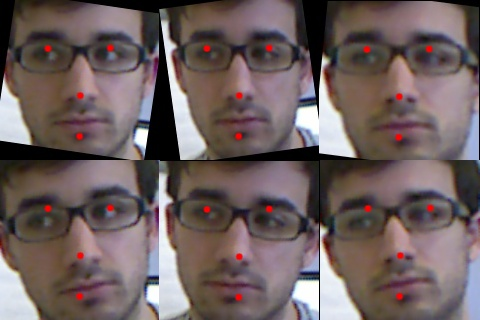
\includegraphics[width=1.0\textwidth]{../img/norm_geometric.jpg}
\caption{This figure depicts a set of three images, that have been processed by the geometrical normalization
algorithm. The artificially added red dots show the norm positions of eyes, nose and mouth.}
\label{fig:NormFace}
\end{figure}
Figure \ref{fig:NormFace} shows that by the geometrical normalization the misalignment of faces due to a varying head pose 
can be overcome or at least minimized.


\subsection{Geometric normalization with depth information}
When there is depth information available for the face image, one is able to use this information for the warping transformation.

\begin{itemize}
\item Get points in point cloud, that correspond to the detected face features
\item Calculate the pose and position of a virtual camera with respect to the 3D points and the norm previos
ly determined norm coordinates of the face features.
\item Resample the pointcloud (RGBXYZ) from the calculated pnp
\item Filter resulting image to compensate for occlusions and poorly sampled pointcloud in image regions
\end{itemize}



